% Data Science Lab talk
% build: pdflatex plant3d.tex && pdflatex plant3d.tex
\documentclass[aspectratio=169,11pt]{beamer}

\usepackage[T1]{fontenc}
\usepackage[utf8]{inputenc}
\usepackage{tgheros}
\renewcommand*\familydefault{\sfdefault}
\renewcommand*\ttdefault{lmtt}
\usepackage{microtype}
\usepackage{tikz}
\usetikzlibrary{arrows.meta,positioning,shapes.geometric,fit,backgrounds}

% --------------------------------------------------------------- 1
% Colours taken from the unibe.ch corporate stylesheet,
% arranged for a dark background.
% --------------------------------------------------------------- 2
\definecolor{ubBg}{HTML}{121212}        % --color-black
\definecolor{ubSurface}{HTML}{1C1C1C}
\definecolor{ubAnthrazit}{HTML}{262626} % --color-anthrazit
\definecolor{ubRed}{HTML}{FF0033}       % --color-red-logo
\definecolor{ubRedDark}{HTML}{D6002B}   % --color-red
\definecolor{ubBlue}{HTML}{2D98E0}      % --color-link-negative
\definecolor{ubGreen}{HTML}{11922D}     % --color-green
\definecolor{ubYellow}{HTML}{FFAD00}    % --color-yellow
\definecolor{ubText}{HTML}{E5E5E5}      % --color-grey-light
\definecolor{ubMuted}{HTML}{999999}     % --color-grey-mid-darker
\definecolor{ubGreyDark}{HTML}{464646}  % --color-grey-dark
\definecolor{ubPanel}{HTML}{171717}

\usetheme{default}
\setbeamertemplate{navigation symbols}{}

\setbeamercolor{background canvas}{bg=ubBg}
\setbeamercolor{normal text}{fg=ubText,bg=ubBg}
\setbeamercolor{structure}{fg=ubRed}
\setbeamercolor{frametitle}{fg=white,bg=ubBg}
\setbeamercolor{title}{fg=white}
\setbeamercolor{alerted text}{fg=ubRed}
\setbeamercolor{itemize item}{fg=ubRed}
\setbeamercolor{itemize subitem}{fg=ubMuted}
\setbeamercolor{enumerate item}{fg=ubRed}
\setbeamercolor{footline}{fg=ubMuted,bg=ubBg}
\setbeamercolor{codebox}{fg=ubText,bg=ubSurface}
\setbeamercolor{notebox}{fg=ubText,bg=ubAnthrazit}

\setbeamerfont{frametitle}{size=\Large,series=\bfseries}
\setbeamerfont{title}{size=\huge,series=\bfseries}
\setbeamerfont{footline}{size=\scriptsize}

\setbeamertemplate{itemize item}{\raisebox{0.15ex}{\scriptsize$\blacksquare$}}
\setbeamertemplate{itemize subitem}{\raisebox{0.15ex}{\tiny$\blacksquare$}}
\setbeamertemplate{enumerate item}{\color{ubRed}\bfseries\insertenumlabel.}

\setbeamertemplate{frametitle}{%
  \vspace*{1.0em}%
  \begin{beamercolorbox}[wd=\paperwidth,leftskip=0.9cm,rightskip=0.9cm]{frametitle}%
    \usebeamerfont{frametitle}\insertframetitle\par
    \vskip4pt
    {\color{ubRed}\rule{2.4em}{2.2pt}}
  \end{beamercolorbox}%
  \vspace*{0.4em}%
}

\setbeamertemplate{footline}{%
  \hbox{%
  \begin{beamercolorbox}[wd=\paperwidth,ht=2.6ex,dp=1.6ex,leftskip=0.9cm,rightskip=0.9cm]{footline}%
    \usebeamerfont{footline}Data Science Lab\quad\textbar\quad University of Bern%
    \hfill%
    {\color{ubRed}\bfseries\insertframenumber}%
  \end{beamercolorbox}}%
}

\setbeamertemplate{section page}{%
  \begin{center}
    {\color{ubRed}\bfseries\Huge\insertsectionnumber}\\[0.6em]
    {\color{white}\bfseries\Large\insertsectionhead}\\[0.5em]
    {\color{ubRed}\rule{3em}{2.2pt}}
  \end{center}
}
\AtBeginSection[]{%
  \begin{frame}[plain]
    \vfill\usebeamertemplate{section page}\vfill
  \end{frame}%
}

% helpers -------------------------------------------------------
\newenvironment{codebox}
  {\begin{beamercolorbox}[wd=\dimexpr\textwidth-16pt\relax,sep=7pt]{codebox}\ttfamily\footnotesize}
  {\end{beamercolorbox}}
\newenvironment{notebox}
  {\begin{beamercolorbox}[wd=\dimexpr\textwidth-16pt\relax,sep=8pt]{notebox}\small}
  {\end{beamercolorbox}}
\newcommand{\badge}[2]{{\setlength{\fboxsep}{3pt}\colorbox{#1}{\color{white}\bfseries\footnotesize\strut #2}}}
\newcommand{\key}[1]{{\color{ubBlue}\ttfamily #1}}
\newcommand{\hi}[1]{{\color{ubRed}\bfseries #1}}

\title{Programmatic Access to University Compute Resources}
\subtitle{Using UBELIX and GPUStack in a software project}
\author{David Herrmann \quad\textbar\quad Sebastian Flick}
\institute{Data Science Lab, University of Bern}
\date{Data Talk}

\begin{document}

% --------------------------------------------------------------- 3
\begin{frame}[plain]
  \vspace{1.2em}
  {\color{ubRed}\rule{4em}{3pt}}\par
  \vspace{0.8em}
  {\usebeamerfont{title}\color{white}\inserttitle}\par
  \vspace{0.7em}
  {\color{ubText}\large\insertsubtitle}\par
  \vspace{1.6em}
  {\color{ubText}\insertauthor}\par
  \vspace{0.3em}
  {\color{ubMuted}\small\insertinstitute}\par
  \vspace{0.2em}
  {\color{ubMuted}\small\insertdate}
\end{frame}

% --------------------------------------------------------------- 5
\begin{frame}{The project}
  \begin{itemize}\setlength\itemsep{0.7em}
    \item \key{plant3d}: film a plant $\rightarrow$ 3D model in the browser
    \item Reconstruction is Gaussian splatting (requires a GPU)
    \item Eleven metadata fields per recording, typed in a greenhouse, on a phone
    \item We want to record what people say while they film to extract metadata
  \end{itemize}
  \vspace{1.1em}
  \begin{notebox}
    All of this should ideally be done in-house.
  \end{notebox}
\end{frame}

% --------------------------------------------------------------- 6
\begin{frame}{Three problems}
  \begin{enumerate}\setlength\itemsep{1.0em}
    \item Speech to text\\
      {\small\color{ubMuted}the words out of the recording}
    \item Text to metadata\\
      {\small\color{ubMuted}eleven fields out of the words}
    \item Programmatic access to UBELIX\\
      {\small\color{ubMuted}the cluster has no API}
  \end{enumerate}
\end{frame}

\section{Speech to text}

% --------------------------------------------------------------- 8
\begin{frame}{Try decoding locally, fail over to the server}
  \begin{itemize}\setlength\itemsep{0.55em}
    \item The model needs the audio. The video is up to 500 MB.
    \item Web Audio API: decode, downmix, resample $\rightarrow$ a few hundred kB
    \item Some browsers do not provide that API
    \item On failure, \key{ffmpeg} extracts the audio on the server
  \end{itemize}
  \vspace{0.6em}
  \begin{codebox}
    \color{ubMuted}try \{\color{ubText}\\
    \hspace*{1em}transcriptionFile = await extractAudioFromVideo(file);\\
    \color{ubMuted}\} catch \{\color{ubText}\\
    \hspace*{1em}usedVideoFallback = true;\hspace*{1em}\color{ubMuted}// let the server do it\color{ubText}\\
    \color{ubMuted}\}
  \end{codebox}
\end{frame}

% --------------------------------------------------------------- 9
\begin{frame}{GPUStack existed}
  \begin{itemize}\setlength\itemsep{0.8em}
    \item Initially, the only feasible option seemed to be a subscription (contract, research data leaving the university).
    \item Then we learned about \key{gpustack.unibe.ch}
    \item University hardware, free for members, OpenAI-compatible
    \item \key{faster-whisper-large-v3} for the transcript. One URL, one token.
  \end{itemize}
  \vspace{1.0em}
  \begin{notebox}
    The university's GPUStack provides various reasonably up-to-date GenAI models.
  \end{notebox}
\end{frame}

\section{Text to metadata}

% --------------------------------------------------------------- 11
\begin{frame}{From transcript to form}
  \vspace{0.1em}\par
  {\small\color{ubMuted}transcript $\rightarrow$ \key{gpt-oss-120b}, same GPUStack
   $\rightarrow$ eleven fields}
  \vspace{0.7em}
  \begin{columns}[t]
    \begin{column}{0.47\textwidth}
      \vspace{0pt}
      \begin{codebox}
        "Maize, cultivar Ronaldinio,\\
        three weeks, still vegetative,\\
        greenhouse, two litre pots,\\
        standard soil. Operator Anna."
      \end{codebox}
    \end{column}
    \begin{column}{0.47\textwidth}
      \vspace{0pt}
      \begin{codebox}
        species: \color{ubBlue}Zea mays\color{ubText}\\
        cultivar: \color{ubBlue}Ronaldinio\color{ubText}\\
        plant\_age: \color{ubBlue}3 weeks\color{ubText}\\
        pot\_volume: \color{ubBlue}2\color{ubText}\\
        operator: \color{ubBlue}Anna\color{ubText}\\
        genotype: \color{ubMuted}null
      \end{codebox}
    \end{column}
  \end{columns}
  \vspace{0.7em}
  {\small\color{ubMuted}Prompt does the work: only the JSON object, unknown
  fields null, \key{temperature 0}. Form stays editable.}
  \vspace{0.4em}\par
  \hi{Demo}
\end{frame}

% --------------------------------------------------------------- 12
\begin{frame}{The prompt}
  \begin{codebox}
    \scriptsize
    System:\\
    You translate natural language descriptions of plant experiments\\
    into a JSON object with the following format:\\
    \color{ubMuted}\{ "type": "object", "properties": \{\\
    ~~~~"title":~~~~~~\{"type": "string", "description": "A short descriptive title"\},\\
    ~~~~"species":~~~~\{"type": "string", "description": "Plant species name"\},\\
    ~~~~"cultivar":~~~\{"type": "string", "description": "Plant cultivar or variety"\},\\
    ~~~~"plant\_age":~~\{"type": "string", "description": "Age of the plant"\},\\
    ~~~~"pot\_volume":~\{"type": "number", "description": "Volume of the pot in liters"\},\\
    ~~~~... genotype, growth stage, environment, substrate, treatments, operator\\
    ~~\}, "additionalProperties": false \}\color{ubText}\\[0.15em]
    Rules:\\
    - ONLY output the json object, do not include any explanations or extra text.\\
    - If information is missing or uncertain, make the field null.
  \end{codebox}
  \vspace{0.1em}
  {\small\color{ubMuted}The schema is trimmed here, the rest is the prompt as it
  ships. \key{temperature 0}, and \key{<think>} blocks get stripped before we parse.}
\end{frame}

\section{Programmatic access to UBELIX}

% --------------------------------------------------------------- 13
\begin{frame}{UBELIX has no side door}
  \begin{itemize}\setlength\itemsep{0.8em}
    \item How people use it today: SSH in, write a batch script, type \key{sbatch},
      come back later
    \item A workflow for a person at a terminal
    \item No API, no tokens, no webhooks
  \end{itemize}
  \vspace{1.2em}
  \begin{notebox}
    We asked around, nobody had done it from an application.
  \end{notebox}
\end{frame}

% --------------------------------------------------------------- 14
\begin{frame}{So we use the front door}
  \begin{itemize}\setlength\itemsep{0.55em}
    \item Service account, own ed25519 key
    \item \key{paramiko}: SSH library for Python
    \item \key{sbatch --parsable} produces (parseable) JSON output $\rightarrow$ read job id
    \item \key{sacct --json} again JSON output $\rightarrow$ extract current processing status
    \item Four concurrent workers submit jobs over SSH and poll their ID
  \end{itemize}
  \vspace{1.0em}
  \begin{center}
    \badge{ubGreyDark}{PENDING}\hspace{0.7em}
    \badge{ubYellow}{PROCESSING}\hspace{0.7em}
    \badge{ubGreen}{PROCESSED}\hspace{0.7em}
    \badge{ubRedDark}{FAILED}
  \end{center}
\end{frame}

% --------------------------------------------------------------- 15
\begin{frame}{The whole path}
  \begin{center}
  \resizebox{0.94\textwidth}{!}{%
  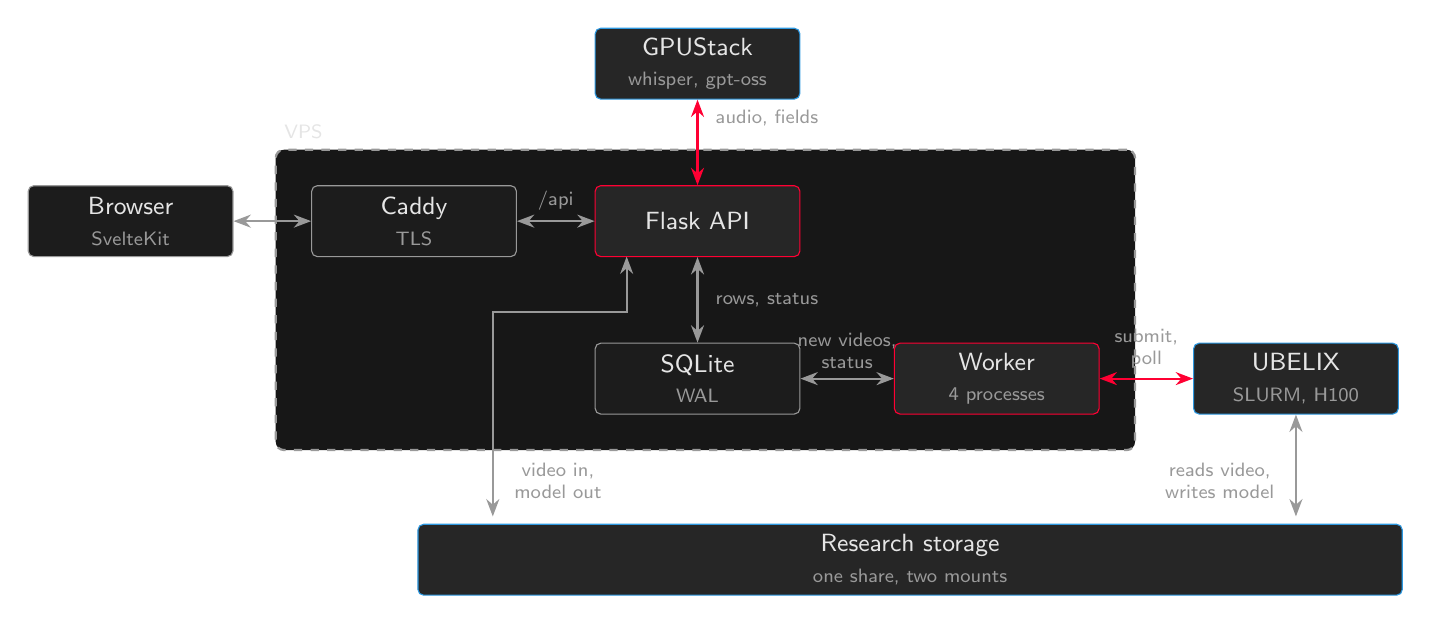
\begin{tikzpicture}[
      font=\small,
      box/.style={draw=ubMuted,fill=ubSurface,text=ubText,rounded corners=2pt,
                  minimum height=9mm,minimum width=26mm,align=center,inner sep=3pt},
      hot/.style={box,draw=ubRed,fill=ubAnthrazit},
      ext/.style={box,draw=ubBlue,fill=ubAnthrazit},
      b/.style={{Stealth[length=2.2mm]}-{Stealth[length=2.2mm]},draw=ubMuted,thick},
      br/.style={{Stealth[length=2.2mm]}-{Stealth[length=2.2mm]},draw=ubRed,thick},
      lbl/.style={text=ubMuted,font=\scriptsize,align=center}
    ]
    \node[box] (browser)  at ( 0.0, 0.0) {Browser\\{\color{ubMuted}\scriptsize SvelteKit}};
    \node[box] (caddy)    at ( 3.6, 0.0) {Caddy\\{\color{ubMuted}\scriptsize TLS}};
    \node[hot] (api)      at ( 7.2, 0.0) {Flask API};
    \node[ext] (gpustack) at ( 7.2, 2.0) {GPUStack\\{\color{ubMuted}\scriptsize whisper, gpt-oss}};

    \node[box] (db)       at ( 7.2,-2.0) {SQLite\\{\color{ubMuted}\scriptsize WAL}};
    \node[hot] (worker)   at (11.0,-2.0) {Worker\\{\color{ubMuted}\scriptsize 4 processes}};
    \node[ext] (ubelix)   at (14.8,-2.0) {UBELIX\\{\color{ubMuted}\scriptsize SLURM, H100}};

    \node[ext,minimum width=125mm] (store) at (9.9,-4.3)
      {Research storage\\{\color{ubMuted}\scriptsize one share, two mounts}};

    % everything inside this box is one VPS, four containers on a bridge network
    \begin{scope}[on background layer]
      \node[draw=ubMuted,dashed,thick,rounded corners=3pt,inner sep=4.5mm,
            fill=ubPanel,fit=(caddy)(api)(db)(worker)] (vps) {};
    \end{scope}
    \node[lbl,anchor=south west,text=ubText] at (vps.north west) {VPS};

    \draw[b]  (browser) -- (caddy);
    \draw[b]  (caddy)   -- node[lbl,above]{/api} (api);
    \draw[br] (api)     -- node[lbl,right,xshift=1mm,pos=0.78]{audio, fields} (gpustack);

    \draw[b]  (api)     -- node[lbl,right,xshift=1mm]{rows, status} (db);
    \draw[b]  (db)      -- node[lbl,above]{new videos,\\status} (worker);
    \draw[br] (worker)  -- node[lbl,above]{submit,\\poll} (ubelix);

    \draw[b]  (6.3,-0.45) -- (6.3,-1.15) -- (4.6,-1.15) -- (4.6,-3.75);
    \node[lbl,right] at (4.75,-3.3) {video in,\\model out};

    \draw[b]  (ubelix.south) -- (14.8,-3.75);
    \node[lbl,left] at (14.65,-3.3) {reads video,\\writes model};
  \end{tikzpicture}}
  \end{center}
  \vspace{0.25em}
  {\small\color{ubMuted}Four containers on one host. Only the proxy has a port open.}
\end{frame}

% --------------------------------------------------------------- 14
\begin{frame}{What we take away}
  \begin{enumerate}\setlength\itemsep{1.0em}
    \item Ask what the university already runs. GPUStack has LLMs, Speech-to-Text models and Embedding models.
    \item Even though UBELIX doesn't have a web API, service account plus \key{--json} gets far.
  \end{enumerate}
\end{frame}

% --------------------------------------------------------------- 15
\begin{frame}[plain]
  \vfill
  \begin{center}
    {\color{ubRed}\rule{3em}{2.5pt}}\\[0.8em]
    {\color{white}\Huge\bfseries Thank you}\\[1.0em]
    {\color{ubText}\large plant3d.ips.unibe.ch}\\[0.4em]
    {\color{ubMuted}David Herrmann \quad\textbar\quad Sebastian Flick}
  \end{center}
  \vfill
\end{frame}

\end{document}
